% Options for packages loaded elsewhere
\PassOptionsToPackage{unicode}{hyperref}
\PassOptionsToPackage{hyphens}{url}
%
\documentclass[
]{article}
\usepackage{lmodern}
\usepackage{amssymb,amsmath}
\usepackage{ifxetex,ifluatex}
\ifnum 0\ifxetex 1\fi\ifluatex 1\fi=0 % if pdftex
  \usepackage[T1]{fontenc}
  \usepackage[utf8]{inputenc}
  \usepackage{textcomp} % provide euro and other symbols
\else % if luatex or xetex
  \usepackage{unicode-math}
  \defaultfontfeatures{Scale=MatchLowercase}
  \defaultfontfeatures[\rmfamily]{Ligatures=TeX,Scale=1}
\fi
% Use upquote if available, for straight quotes in verbatim environments
\IfFileExists{upquote.sty}{\usepackage{upquote}}{}
\IfFileExists{microtype.sty}{% use microtype if available
  \usepackage[]{microtype}
  \UseMicrotypeSet[protrusion]{basicmath} % disable protrusion for tt fonts
}{}
\makeatletter
\@ifundefined{KOMAClassName}{% if non-KOMA class
  \IfFileExists{parskip.sty}{%
    \usepackage{parskip}
  }{% else
    \setlength{\parindent}{0pt}
    \setlength{\parskip}{6pt plus 2pt minus 1pt}}
}{% if KOMA class
  \KOMAoptions{parskip=half}}
\makeatother
\usepackage{xcolor}
\IfFileExists{xurl.sty}{\usepackage{xurl}}{} % add URL line breaks if available
\IfFileExists{bookmark.sty}{\usepackage{bookmark}}{\usepackage{hyperref}}
\hypersetup{
  hidelinks,
  pdfcreator={LaTeX via pandoc}}
\urlstyle{same} % disable monospaced font for URLs
\usepackage[margin=1in]{geometry}
\usepackage{color}
\usepackage{fancyvrb}
\newcommand{\VerbBar}{|}
\newcommand{\VERB}{\Verb[commandchars=\\\{\}]}
\DefineVerbatimEnvironment{Highlighting}{Verbatim}{commandchars=\\\{\}}
% Add ',fontsize=\small' for more characters per line
\usepackage{framed}
\definecolor{shadecolor}{RGB}{248,248,248}
\newenvironment{Shaded}{\begin{snugshade}}{\end{snugshade}}
\newcommand{\AlertTok}[1]{\textcolor[rgb]{0.94,0.16,0.16}{#1}}
\newcommand{\AnnotationTok}[1]{\textcolor[rgb]{0.56,0.35,0.01}{\textbf{\textit{#1}}}}
\newcommand{\AttributeTok}[1]{\textcolor[rgb]{0.77,0.63,0.00}{#1}}
\newcommand{\BaseNTok}[1]{\textcolor[rgb]{0.00,0.00,0.81}{#1}}
\newcommand{\BuiltInTok}[1]{#1}
\newcommand{\CharTok}[1]{\textcolor[rgb]{0.31,0.60,0.02}{#1}}
\newcommand{\CommentTok}[1]{\textcolor[rgb]{0.56,0.35,0.01}{\textit{#1}}}
\newcommand{\CommentVarTok}[1]{\textcolor[rgb]{0.56,0.35,0.01}{\textbf{\textit{#1}}}}
\newcommand{\ConstantTok}[1]{\textcolor[rgb]{0.00,0.00,0.00}{#1}}
\newcommand{\ControlFlowTok}[1]{\textcolor[rgb]{0.13,0.29,0.53}{\textbf{#1}}}
\newcommand{\DataTypeTok}[1]{\textcolor[rgb]{0.13,0.29,0.53}{#1}}
\newcommand{\DecValTok}[1]{\textcolor[rgb]{0.00,0.00,0.81}{#1}}
\newcommand{\DocumentationTok}[1]{\textcolor[rgb]{0.56,0.35,0.01}{\textbf{\textit{#1}}}}
\newcommand{\ErrorTok}[1]{\textcolor[rgb]{0.64,0.00,0.00}{\textbf{#1}}}
\newcommand{\ExtensionTok}[1]{#1}
\newcommand{\FloatTok}[1]{\textcolor[rgb]{0.00,0.00,0.81}{#1}}
\newcommand{\FunctionTok}[1]{\textcolor[rgb]{0.00,0.00,0.00}{#1}}
\newcommand{\ImportTok}[1]{#1}
\newcommand{\InformationTok}[1]{\textcolor[rgb]{0.56,0.35,0.01}{\textbf{\textit{#1}}}}
\newcommand{\KeywordTok}[1]{\textcolor[rgb]{0.13,0.29,0.53}{\textbf{#1}}}
\newcommand{\NormalTok}[1]{#1}
\newcommand{\OperatorTok}[1]{\textcolor[rgb]{0.81,0.36,0.00}{\textbf{#1}}}
\newcommand{\OtherTok}[1]{\textcolor[rgb]{0.56,0.35,0.01}{#1}}
\newcommand{\PreprocessorTok}[1]{\textcolor[rgb]{0.56,0.35,0.01}{\textit{#1}}}
\newcommand{\RegionMarkerTok}[1]{#1}
\newcommand{\SpecialCharTok}[1]{\textcolor[rgb]{0.00,0.00,0.00}{#1}}
\newcommand{\SpecialStringTok}[1]{\textcolor[rgb]{0.31,0.60,0.02}{#1}}
\newcommand{\StringTok}[1]{\textcolor[rgb]{0.31,0.60,0.02}{#1}}
\newcommand{\VariableTok}[1]{\textcolor[rgb]{0.00,0.00,0.00}{#1}}
\newcommand{\VerbatimStringTok}[1]{\textcolor[rgb]{0.31,0.60,0.02}{#1}}
\newcommand{\WarningTok}[1]{\textcolor[rgb]{0.56,0.35,0.01}{\textbf{\textit{#1}}}}
\usepackage{graphicx,grffile}
\makeatletter
\def\maxwidth{\ifdim\Gin@nat@width>\linewidth\linewidth\else\Gin@nat@width\fi}
\def\maxheight{\ifdim\Gin@nat@height>\textheight\textheight\else\Gin@nat@height\fi}
\makeatother
% Scale images if necessary, so that they will not overflow the page
% margins by default, and it is still possible to overwrite the defaults
% using explicit options in \includegraphics[width, height, ...]{}
\setkeys{Gin}{width=\maxwidth,height=\maxheight,keepaspectratio}
% Set default figure placement to htbp
\makeatletter
\def\fps@figure{htbp}
\makeatother
\setlength{\emergencystretch}{3em} % prevent overfull lines
\providecommand{\tightlist}{%
  \setlength{\itemsep}{0pt}\setlength{\parskip}{0pt}}
\setcounter{secnumdepth}{-\maxdimen} % remove section numbering

\author{}
\date{\vspace{-2.5em}}

\begin{document}

\hypertarget{inferential-data-analysis}{%
\section{Inferential Data Analysis}\label{inferential-data-analysis}}

\hypertarget{loading-the-data-set-and-basic-exploratory-analysis}{%
\subsection{Loading the Data Set and Basic Exploratory
Analysis}\label{loading-the-data-set-and-basic-exploratory-analysis}}

\begin{Shaded}
\begin{Highlighting}[]
\NormalTok{data =}\StringTok{ }\NormalTok{ToothGrowth}
\KeywordTok{library}\NormalTok{(ggplot2)}
\NormalTok{g =}\StringTok{ }\KeywordTok{ggplot}\NormalTok{(data,}\KeywordTok{aes}\NormalTok{(supp,len))}
\KeywordTok{qplot}\NormalTok{(dose,len,}\DataTypeTok{data =}\NormalTok{ data,}\DataTypeTok{col =}\NormalTok{ supp)}
\end{Highlighting}
\end{Shaded}

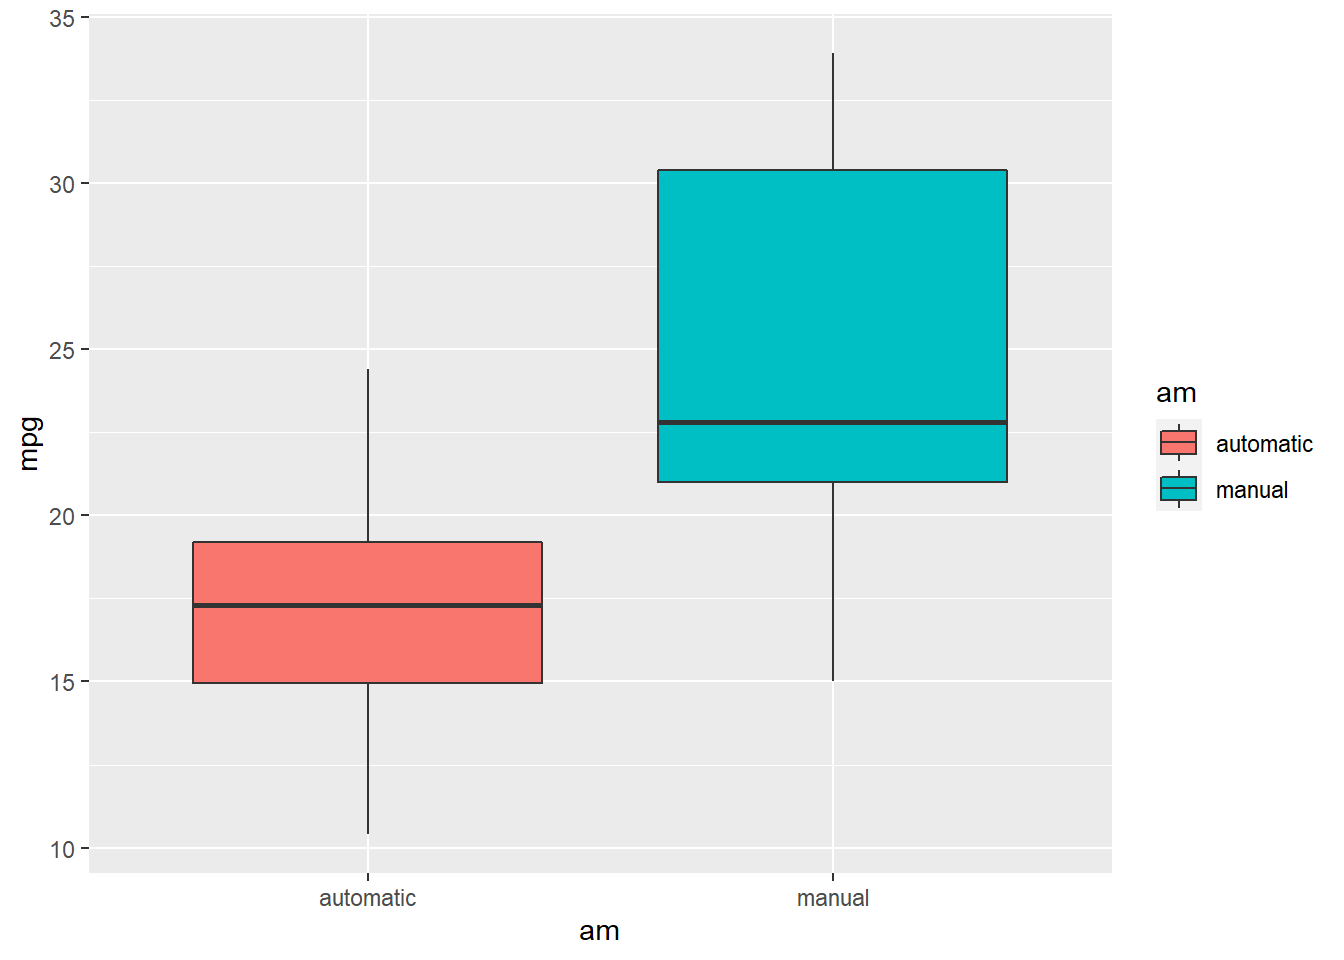
\includegraphics{stats2_files/figure-latex/unnamed-chunk-1-1.pdf}

This plot shows that for two types of supplements measurementa of tooth
length is taken for three different groups.\\
Let's now plot a panel boxplot to get a clear idea of the data.

\begin{Shaded}
\begin{Highlighting}[]
\NormalTok{g}\OperatorTok{+}\KeywordTok{geom_boxplot}\NormalTok{(}\DataTypeTok{color =} \StringTok{"blue"}\NormalTok{)}\OperatorTok{+}\KeywordTok{facet_grid}\NormalTok{(.}\OperatorTok{~}\NormalTok{dose)}
\end{Highlighting}
\end{Shaded}

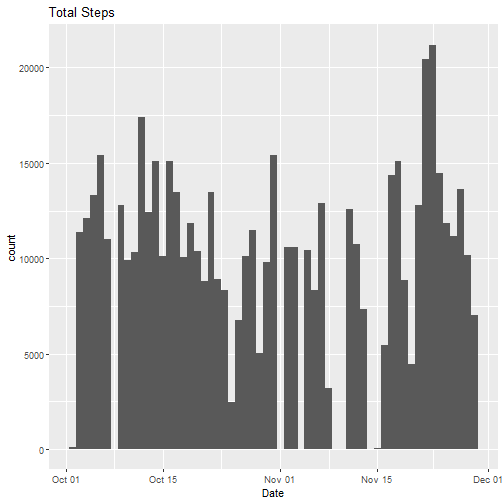
\includegraphics{stats2_files/figure-latex/unnamed-chunk-2-1.pdf}

We can infer from this plot that it would be interesting to analyse the
data dose-wise and compare which supplement was better.\\
Following is the summary of the data dose-wise.

\begin{Shaded}
\begin{Highlighting}[]
\NormalTok{l =}\StringTok{ }\KeywordTok{lapply}\NormalTok{(}\KeywordTok{unique}\NormalTok{(data}\OperatorTok{$}\NormalTok{dose),}\ControlFlowTok{function}\NormalTok{(x) }\KeywordTok{summary}\NormalTok{(}\KeywordTok{subset}\NormalTok{(data,dose}\OperatorTok{==}\NormalTok{x)))}
\KeywordTok{names}\NormalTok{(l) =}\StringTok{ }\KeywordTok{c}\NormalTok{(}\StringTok{"0.5"}\NormalTok{,}\StringTok{"1.0"}\NormalTok{,}\StringTok{"2.0"}\NormalTok{)}
\NormalTok{l}
\end{Highlighting}
\end{Shaded}

\begin{verbatim}
## $`0.5`
##       len         supp         dose    
##  Min.   : 4.200   OJ:10   Min.   :0.5  
##  1st Qu.: 7.225   VC:10   1st Qu.:0.5  
##  Median : 9.850           Median :0.5  
##  Mean   :10.605           Mean   :0.5  
##  3rd Qu.:12.250           3rd Qu.:0.5  
##  Max.   :21.500           Max.   :0.5  
## 
## $`1.0`
##       len        supp         dose  
##  Min.   :13.60   OJ:10   Min.   :1  
##  1st Qu.:16.25   VC:10   1st Qu.:1  
##  Median :19.25           Median :1  
##  Mean   :19.73           Mean   :1  
##  3rd Qu.:23.38           3rd Qu.:1  
##  Max.   :27.30           Max.   :1  
## 
## $`2.0`
##       len        supp         dose  
##  Min.   :18.50   OJ:10   Min.   :2  
##  1st Qu.:23.52   VC:10   1st Qu.:2  
##  Median :25.95           Median :2  
##  Mean   :26.10           Mean   :2  
##  3rd Qu.:27.82           3rd Qu.:2  
##  Max.   :33.90           Max.   :2
\end{verbatim}

\hypertarget{confidence-intervals-for-different-doses}{%
\subsection{Confidence Intervals for different
Doses}\label{confidence-intervals-for-different-doses}}

Lets analyse this dataset for different doses and compare which
supplement resulted in longer tooth length.\\
FOr this let's do the two groups t-statistic analysis for different
doses and check the confidence interval of the difference of the mean of
the two groups, or in other words test the alternate hypothesis of
unequal mean with the null hypothesis of equal mean.

\begin{Shaded}
\begin{Highlighting}[]
\NormalTok{l =}\StringTok{ }\KeywordTok{lapply}\NormalTok{(}\KeywordTok{c}\NormalTok{(}\FloatTok{0.5}\NormalTok{,}\DecValTok{1}\NormalTok{,}\DecValTok{2}\NormalTok{),}\ControlFlowTok{function}\NormalTok{(x) }\KeywordTok{t.test}\NormalTok{(len}\OperatorTok{~}\NormalTok{supp,}\DataTypeTok{data =} \KeywordTok{subset}\NormalTok{(data,dose }\OperatorTok{==}\StringTok{ }\NormalTok{x),}\DataTypeTok{paired =}\NormalTok{ F,}\DataTypeTok{var.equal =}\NormalTok{ F)}\OperatorTok{$}\NormalTok{conf)}
\KeywordTok{names}\NormalTok{(l) =}\StringTok{ }\KeywordTok{c}\NormalTok{(}\StringTok{"0.5"}\NormalTok{,}\StringTok{"1.0"}\NormalTok{,}\StringTok{"2.0"}\NormalTok{)}
\NormalTok{l}
\end{Highlighting}
\end{Shaded}

\begin{verbatim}
## $`0.5`
## [1] 1.719057 8.780943
## attr(,"conf.level")
## [1] 0.95
## 
## $`1.0`
## [1] 2.802148 9.057852
## attr(,"conf.level")
## [1] 0.95
## 
## $`2.0`
## [1] -3.79807  3.63807
## attr(,"conf.level")
## [1] 0.95
\end{verbatim}

\hypertarget{conslusions}{%
\subsection{Conslusions}\label{conslusions}}

\hypertarget{assumptions}{%
\subsubsection{Assumptions:}\label{assumptions}}

\begin{itemize}
\tightlist
\item
  I have assumed that the two groups are not paired.\\
\item
  Looking at the initial plots, I have also made the assumption of
  unequal variances.
\end{itemize}

\hypertarget{results}{%
\subsubsection{Results:}\label{results}}

\begin{itemize}
\tightlist
\item
  It is clear from the Confidence Interval that for the dose of 0.5 and
  1.0, the interval is positive i.e.~samples with OJ have longer length
  with the confidence of 95\%. Hence, we reject the null hypothesis.\\
\item
  However for 2.0 dose, the interval has both negative and positive
  values of the difference of the mean. Hence we cannot say that they
  perfom differently, in other words we cannot reject the null
  hypothesis.
\end{itemize}

\end{document}
